\chapter{Results}
\label{ch:results}

In this chapter, we first describe our evaluation setup, which consists of the HPC cluster used for our experiments, the matrix datasets, and the algorithmic implementations evaluated. We then present a detailed analysis of various performance metrics, including execution time, memory usage, parallelization and matrix fill-in reduction. 


% In this chapter, you want to show that your implementation meets the objectives.
% Start by briefly describing the type of results you have collected and how these results relate to the objectives.

\section{Evaluation setup}

Everything that is evaluated is ran on Fritz, a high-performance computing cluster at NHR@FAU.

\subsection{Hardware Infrastructure}

Fritz is a parallel CPU cluster operated by NHR@FAU, featuring Intel Ice Lake and Sapphire Rapids processors with an InfiniBand (IB) network and a Lustre-based parallel filesystem accessible under \texttt{\$FASTTMP}. The cluster configuration consists of:
\begin{table}[h]
\centering
\begin{tabular}{|p{1.5cm}|p{4.5cm}|p{2cm}|p{3cm}|}
\hline
\textbf{Nodes} & \textbf{CPUs and Cores} & \textbf{Memory} & \textbf{Slurm Partition} \\
\hline
992 & 2 × Intel Xeon Platinum 8360Y (Ice Lake) & 256 GB & singlenode, multinode \\
  & 2 × 36 cores @2.4 GHz & & \\
\hline
48 & 2 × Intel Xeon Platinum 8470 (Sapphire Rapids) & 1 TB & spr1tb \\
   & 2 × 52 cores @2.0 GHz & & \\
\hline
16 & 2 × Intel Xeon Platinum 8470 (Sapphire Rapids) & 2 TB & spr2tb \\
   & 2 × 52 cores @2.0 GHz & & \\
\hline
\end{tabular}
\caption{Fritz cluster node configuration}
\label{tab:fritz-nodes}
\end{table}

The login nodes fritz[1-4] are equipped with 2 × Intel Xeon Platinum 8360Y (Ice Lake) processors and 512 GB main memory. Additionally, the remote visualization node fviz1 features 2 × Intel Xeon Platinum 8360Y processors with 1 TB main memory, one Nvidia A16 GPU, and 30 TB of local NVMe SSD storage.



% Precisely describe your measurement/evaluation setup in a top-down manner.
% For example:
% \begin{itemize}
%   \item If you used a development platform, which one and how was it configured?
%   \item Which tools did you use?
%   \item What input data set / program / signals / \ldots{} did you use?
%     If your data set is very large, you should fully define and describe it in an appendix chapter and refer to that definition here using simple labels.
%   \item If your implementation is configurable, which configuration(s) did you evaluate?
% \end{itemize}

% The information given here (with references to external work) should be sufficient to reproduce the setup you used for your measurements.

\section{Matrices dataset}

We selected a diverse set of sparse matrices from the SuiteSparse Matrix Collection and our custom dataset of matrices encountered in Quantum Transport to evaluate our implementations. The SuiteSparse matrices chosen are usually which were commonly used in the literature for \textit{METIS} and \textit{SCOTCH} own evaluations. 
[TODO about Quantum transport matrices]


\begin{longtable}{|l|l|r|r|}
\hline
\textbf{Graph name} & \textbf{Group} & \textbf{No. of vertices} & \textbf{No. of edges} \\
\hline
\endfirsthead

\hline
\textbf{Graph name} & \textbf{Group} & \textbf{No. of vertices} & \textbf{No. of edges} \\
\hline
\endhead

\hline
\multicolumn{4}{r}{\textit{Continued on next page}} \\
\endfoot

\hline
\endlastfoot

copter2 & CFD & 55476 & 407714 \\
ex10 & CFD & 2410 & 28625 \\
parabolic\_fem & CFD & 525825 & 2100225 \\
3Dspectralwave & Chemistry & 680943 & 17165766 \\
CO & Chemistry & 221119 & 3943588 \\
crystk03 & Chemistry & 24696 & 887937 \\
Ga19As19H42 & Chemistry & 133123 & 4508981 \\
Si87H76 & Chemistry & 240369 & 5451000 \\
SiH4 & Chemistry & 5041 & 88472 \\
circuit\_3 & Circuit & 12127 & 48137 \\
G2\_circuit & Circuit & 150102 & 438388 \\
memplus & Circuit & 17758 & 126150 \\
rajat06 & Circuit & 10922 & 28922 \\
rajat10 & Circuit & 30202 & 80202 \\
rajat15 & Circuit & 37261 & 443573 \\
144 & Graphs & 144649 & 1074393 \\
598a & Graphs & 110971 & 741934 \\
auto & Graphs & 448695 & 3314611 \\
ca-AstroPh & Graphs & 18772 & 198110 \\
citationCiteseer & Graphs & 268495 & 1156647 \\
delaunay\_n20 & Graphs & 1048576 & 3145686 \\
dictionary28 & Graphs & 52652 & 89038 \\
boyd2 & Optimizations & 466316 & 890091 \\
c-55 & Optimizations & 32780 & 218115 \\
c-70 & Optimizations & 68924 & 363955 \\
gupta2 & Optimizations & 62064 & 2155175 \\
gupta3 & Optimizations & 16783 & 4670105 \\
lpl1 & Optimizations & 32460 & 180248 \\
ncvxbqp1 & Optimizations & 50000 & 199984 \\
apache1 & Structural & 80800 & 311492 \\
apache2 & Structural & 715176 & 2766523 \\
nasasrb & Structural & 54870 & 1366097 \\
\caption{SuiteSparse matrix dataset used for evaluation}
\label{tab:matrix-dataset}
\end{longtable}

\begin{table}[h]
\centering
\caption{Quantum Transport matrix dataset used for evaluation}
\label{tab:qt-matrix-dataset}
\resizebox{\textwidth}{!}{%
\begin{tabular}{|l|r|r|l|}
\hline
\textbf{Graph name} & \textbf{No. of vertices} & \textbf{No. of edges} & \textbf{Description} \\
\hline
airpoll\_conditional\_st3 & 8499 & 1218651 & Spatio-temporal statistical Modelling \\
airpoll\_prior\_st3 & 8499 & 1205931 & Spatio-temporal statistical Modelling \\
cnt\_cp2k & 9152 & 6154350 & DFT Hamiltonian of Carbon Nanotube \\
cnt\_w90 & 768 & 71680 & DFT Hamiltonian of Carbon Nanotube \\
kmc\_potential\_0 & 403605 & 10007089 & Kinetic Monte Carlo for Device Modelling \\
kmc\_potential\_1 & 1632355 & 41208963 & Kinetic Monte Carlo for Device Modelling \\
qubit\_fem\_b4 & 116380 & 2517228 & FEM Matrix for Qubit \\
sinw\_w90 & 7488 & 5310160 & DFT Hamiltonian of Silicon Nanowire \\
\hline
\end{tabular}%
}
\end{table}

\section{Methodology}

For our evaluation, we systematically assessed the performance of eleven different reordering algorithms across all matrices listed in Tables~\ref{tab:matrix-dataset} and~\ref{tab:qt-matrix-dataset}. The evaluated algorithms encompass both sequential and parallel approaches, ranging from classical degree-based methods to graph partitioning and hypergraph-based techniques:

\begin{description}
   \item[\textbf{Classical Methods:}] \mbox{}\\
   \begin{itemize}
      \item \textbf{AMD} -- Approximate Minimum Degree
      \item \textbf{COLAMD} -- Column Approximate Minimum Degree  
      \item \textbf{RCM} -- Reverse Cuthill-McKee
      \item \textbf{Natural} -- Original matrix ordering (baseline)
   \end{itemize}
   
   \item[\textbf{Graph Partitioning Methods:}] \mbox{}\\
   \begin{itemize}
      \item \textbf{METIS} -- Sequential graph partitioning-based reordering
      \item \textbf{METIS+IC} -- METIS with improved coarsening integration
      \item \textbf{SCOTCH} -- Sequential graph partitioning
      \item \textbf{PT-SCOTCH} -- Parallel graph partitioning
      \item \textbf{ParMETIS} -- Parallel graph partitioning
   \end{itemize}
   
   \item[\textbf{Hypergraph-based Methods:}] \mbox{}\\
   \begin{itemize}
      \item \textbf{HG-2, HG-4, HG-8, HG-16} -- Hypergraph-based reordering with block partition sizes of 2, 4, 8, and 16 vertices respectively
   \end{itemize}
\end{description}

The hypergraph-based methods (HG-2, HG-4, HG-8, HG-16) employ different block partition sizes to explore the trade-off between computational complexity and reordering/parallelization quality. All these algorithms are described in detail in Chapter~\ref{ch:background}.

\subsection{Performance Metrics and Measurement Protocol}

Our comprehensive evaluation measures five key performance indicators to assess the effectiveness of each reordering algorithm:

\begin{description}
   \item[\textbf{Fill-in Reduction:}] We measure the number of non-zero entries introduced during symbolic Cholesky factorization using the \texttt{cmpfillin} binary provided by the METIS library. This tool performs symbolic factorization (as described in Chapter~\ref{ch:background}) to count the additional non-zero entries without executing the actual numerical computation. 
      
      \item[\textbf{Computational Complexity:}] We track the total floating-point operation count required for factorization, providing insight into the computational efficiency gains achieved by different reordering strategies.
      
      \item[\textbf{Reordering Time:}] The wall-clock time required to compute the reordering itself is measured using Python's \texttt{time.perf\_counter()} with microsecond precision. This overhead cost is crucial for understanding the practical applicability of each method.
      
      \item[\textbf{Memory Usage:}] We implement a dedicated memory monitoring system using a separate thread that samples memory consumption every 50 milliseconds during reordering operations. The monitoring captures both peak memory usage (maximum RSS observed) and average memory consumption throughout the reordering process. Memory measurements are obtained via the \texttt{psutil} library, tracking the resident set size (RSS) of the process and computing the memory increase relative to a baseline measured before algorithm execution.

      \item[\textbf{Parallelization Potential:}] We assess the elimination tree depth as an indicator of the inherent parallelism available in the factorization. As mentioned in Chapter~\ref{ch:background}, the elimination tree is constructed by identifying parent-child relationships in the symbolic factorization structure, where the tree depth represents the critical path length and thus the theoretical lower bound on parallel factorization time.
\end{description}

For memory profiling, we initially attempted to use the Massif profiler from Valgrind, but encountered issues with our Python-based implementations and the cluster environment. Consequently, we developed a custom memory measurement protocol that employs a thread-safe monitoring system to capture accurate memory usage patterns during reordering operations.

Our memory measurement implementation works by first establishing a baseline memory consumption before starting any reordering algorithm, recording the initial resident set size (RSS) using \texttt{psutil.Process().memory\_info().rss}. During algorithm execution, a dedicated monitoring thread runs concurrently, sampling memory usage every 50 milliseconds throughout the entire operation. This thread continuously updates the maximum observed memory consumption and maintains a comprehensive list of all samples for subsequent average computation.

Upon completion of the reordering algorithm, we compute both the peak memory increase (calculated as the maximum observed RSS minus the baseline) and the average memory increase (computed as the mean of all samples minus the baseline), with results reported in kilobytes. For cases where the monitoring thread fails to capture meaningful data, such as very fast operations that complete before sufficient samples can be collected, we provide conservative estimates based on matrix characteristics, using approximately 10\% of the matrix storage size as an upper bound for memory consumption.

All experiments are executed on the Fritz cluster to ensure consistent hardware conditions across all measurements. Each algorithm is tested on every matrix in our dataset, and results are averaged over five independent runs to mitigate variability. 

\section{Evaluation}

For each matrix in our dataset with different reordering algorithms applied, we have collected all the aforementioned metrics, and these can be found in our appendix/supplementary material \ref{app:experimental_results}. Here, we present results and visualizations for our underlying metrics for some of them.

Figure~\ref{fig:fillin-categories} presents a comparative analysis of fill-in reduction across different matrix categories, showing the ratio of fill-in to original non-zeros for representative matrices from each domain. This visualization demonstrates how reordering effectiveness varies significantly across different problem types and matrix structures.

\begin{figure}[H]
\centering
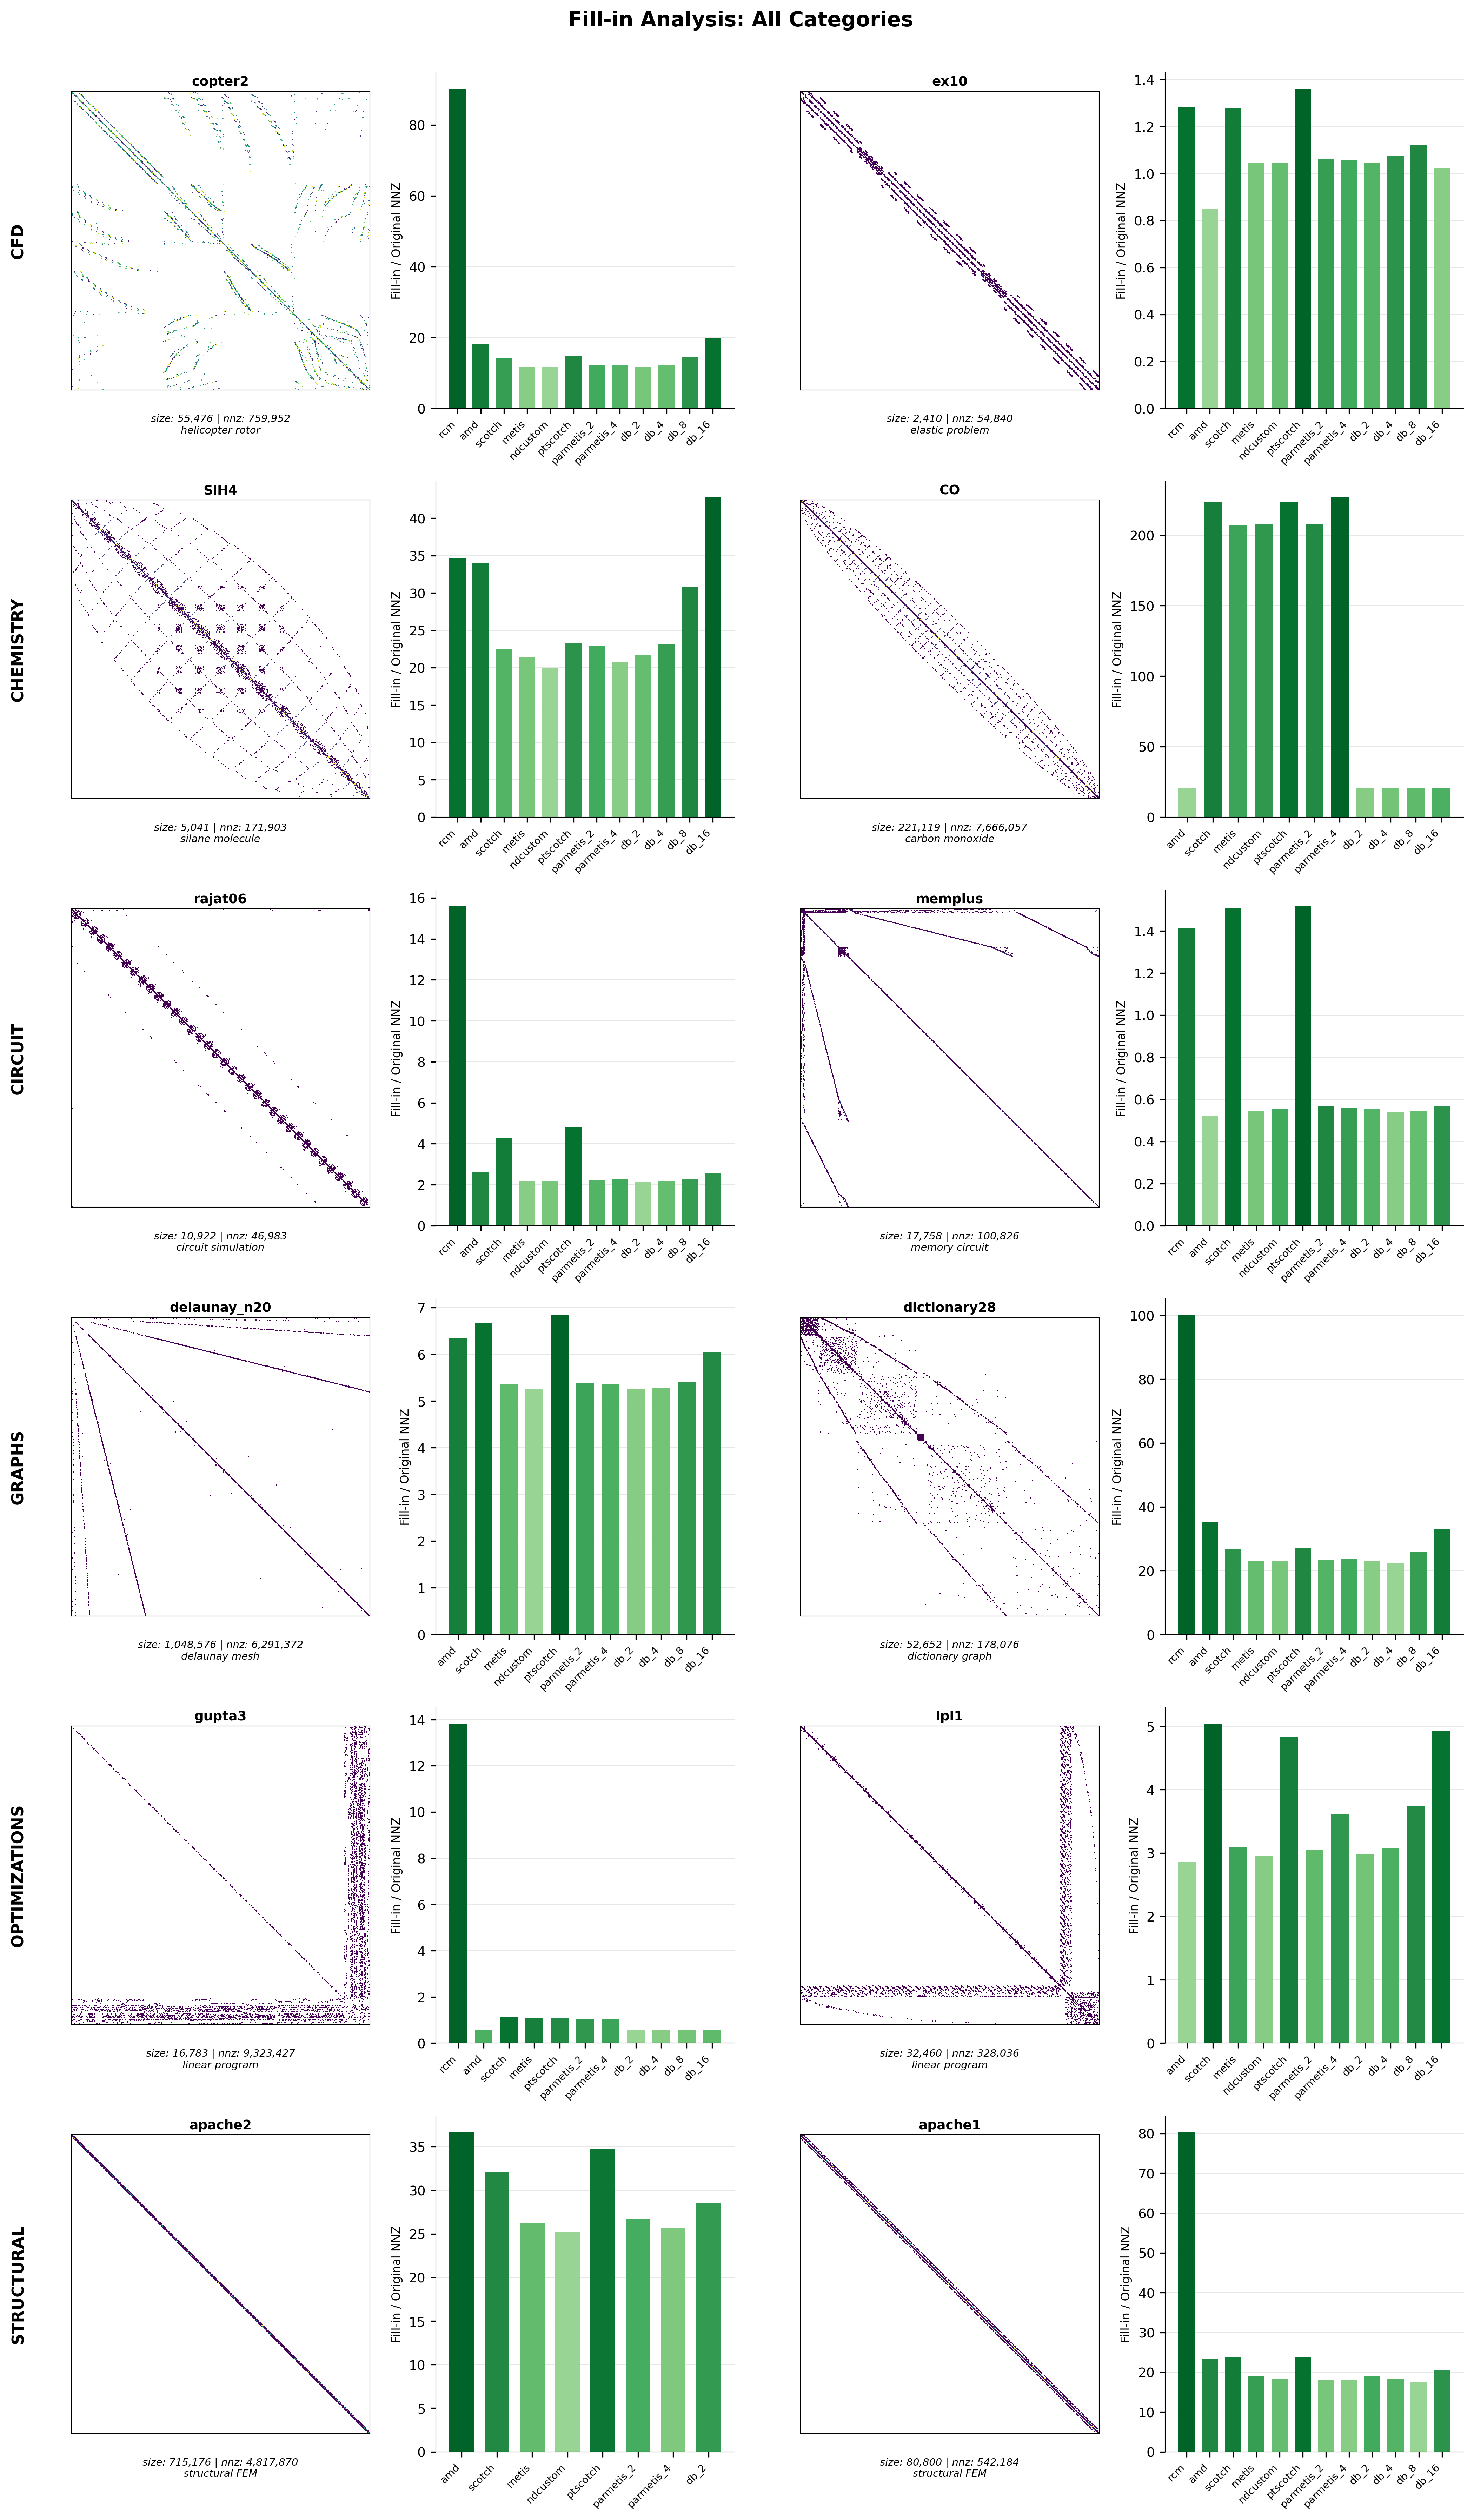
\includegraphics[width=0.9\textwidth]{fig/res/fillin_all_categories.png}
\caption{Fill-in ratio (fill-in/original nnz) comparison across different matrix categories}
\label{fig:fillin-categories}
\end{figure}

Our experimental results reveal distinct performance patterns across different matrix domains and algorithm categories. The hypergraph-based methods, METIS, and our custom METIS implementation with improved coarsening (METIS+IC) consistently emerge as the best-performing approaches, demonstrating better fill-in reduction compared to classical methods. These methods usually achieve 30-60\% lower fill-in values than traditional approaches like AMD and COLAMD across most domains. Among the hypergraph methods, smaller partition sizes (HG-2 and HG-4) typically produce optimal results, while larger partitions are ineffective. Our custom METIS+IC implementation validates the effectiveness of enhanced coarsening strategies by achieving competitive performance with the best hypergraph methods. SCOTCH and PT-SCOTCH show moderate improvements over classical methods but do not match the quality of METIS-based approaches.

Domain-specific analysis reveals that hypergraph methods, METIS, and METIS+IC excel particularly in circuit and graph problems, where they achieve 35-50\% fill-in reduction compared to AMD. For CFD matrices, these advanced methods maintain their superiority with modest but consistent improvements (10-30\%), while chemistry matrices present scalability challenges where many classical methods fail on the largest instances, leaving primarily METIS-based or classical methods viable. The optimization and structural domains show variable performance depending on problem structure, with hypergraph methods and METIS variants providing 10-25\% improvements in most cases.

Figure~\ref{fig:reorder-time-scaling} presents the scaling behavior of reordering algorithms with respect to the number of non-zero entries. This graph shows the time required for each algorithm to complete and how it scales with increasing non-zero counts. 

The reordering time results show notable performance differences across methods. RCM and AMD are the fastest options, with RCM typically completing in under one second (0.006-0.76s) across all matrix sizes and AMD performing well for small-to-medium matrices (0.046-2.09s). SCOTCH and METIS generally complete within reasonable timeframes (under 50 seconds), while parallel methods like ParMETIS and PT-SCOTCH have higher overhead that may be justified for larger problems. The hypergraph partitioning methods (HG variants) require significantly more time, with some executions taking over 270 seconds, which limits their practical applicability for interactive use.

Regarding scalability with increasing NNZ, the methods exhibit different growth patterns. AMD shows sublinear scaling (slope 0.52), which becomes more favorable as matrix size increases, while RCM maintains near-linear scaling (slope 0.72) with consistent performance characteristics. SCOTCH demonstrates reasonable scaling (slope 0.65), and the ParMETIS variants maintain moderate complexity (slopes 0.64-0.68) despite their higher base execution times. METIS+IC shows superlinear scaling (slope 1.14) due to its modified coarsening approach, which becomes problematic for very large matrices, while METIS approaches linear scaling (slope 0.81). The HG hypergraph methods show scaling slopes between 0.71-0.76, though their high absolute execution times remain a concern.

The results indicate that simpler methods like AMD and RCM often provide better practical performance than more complex approaches for large-scale sparse matrix reordering. While parallel methods may become advantageous for extremely large problems, the hypergraph partitioning approaches appear computationally expensive relative to their benefits in typical sparse matrix applications.


\begin{figure}[h!]
\centering
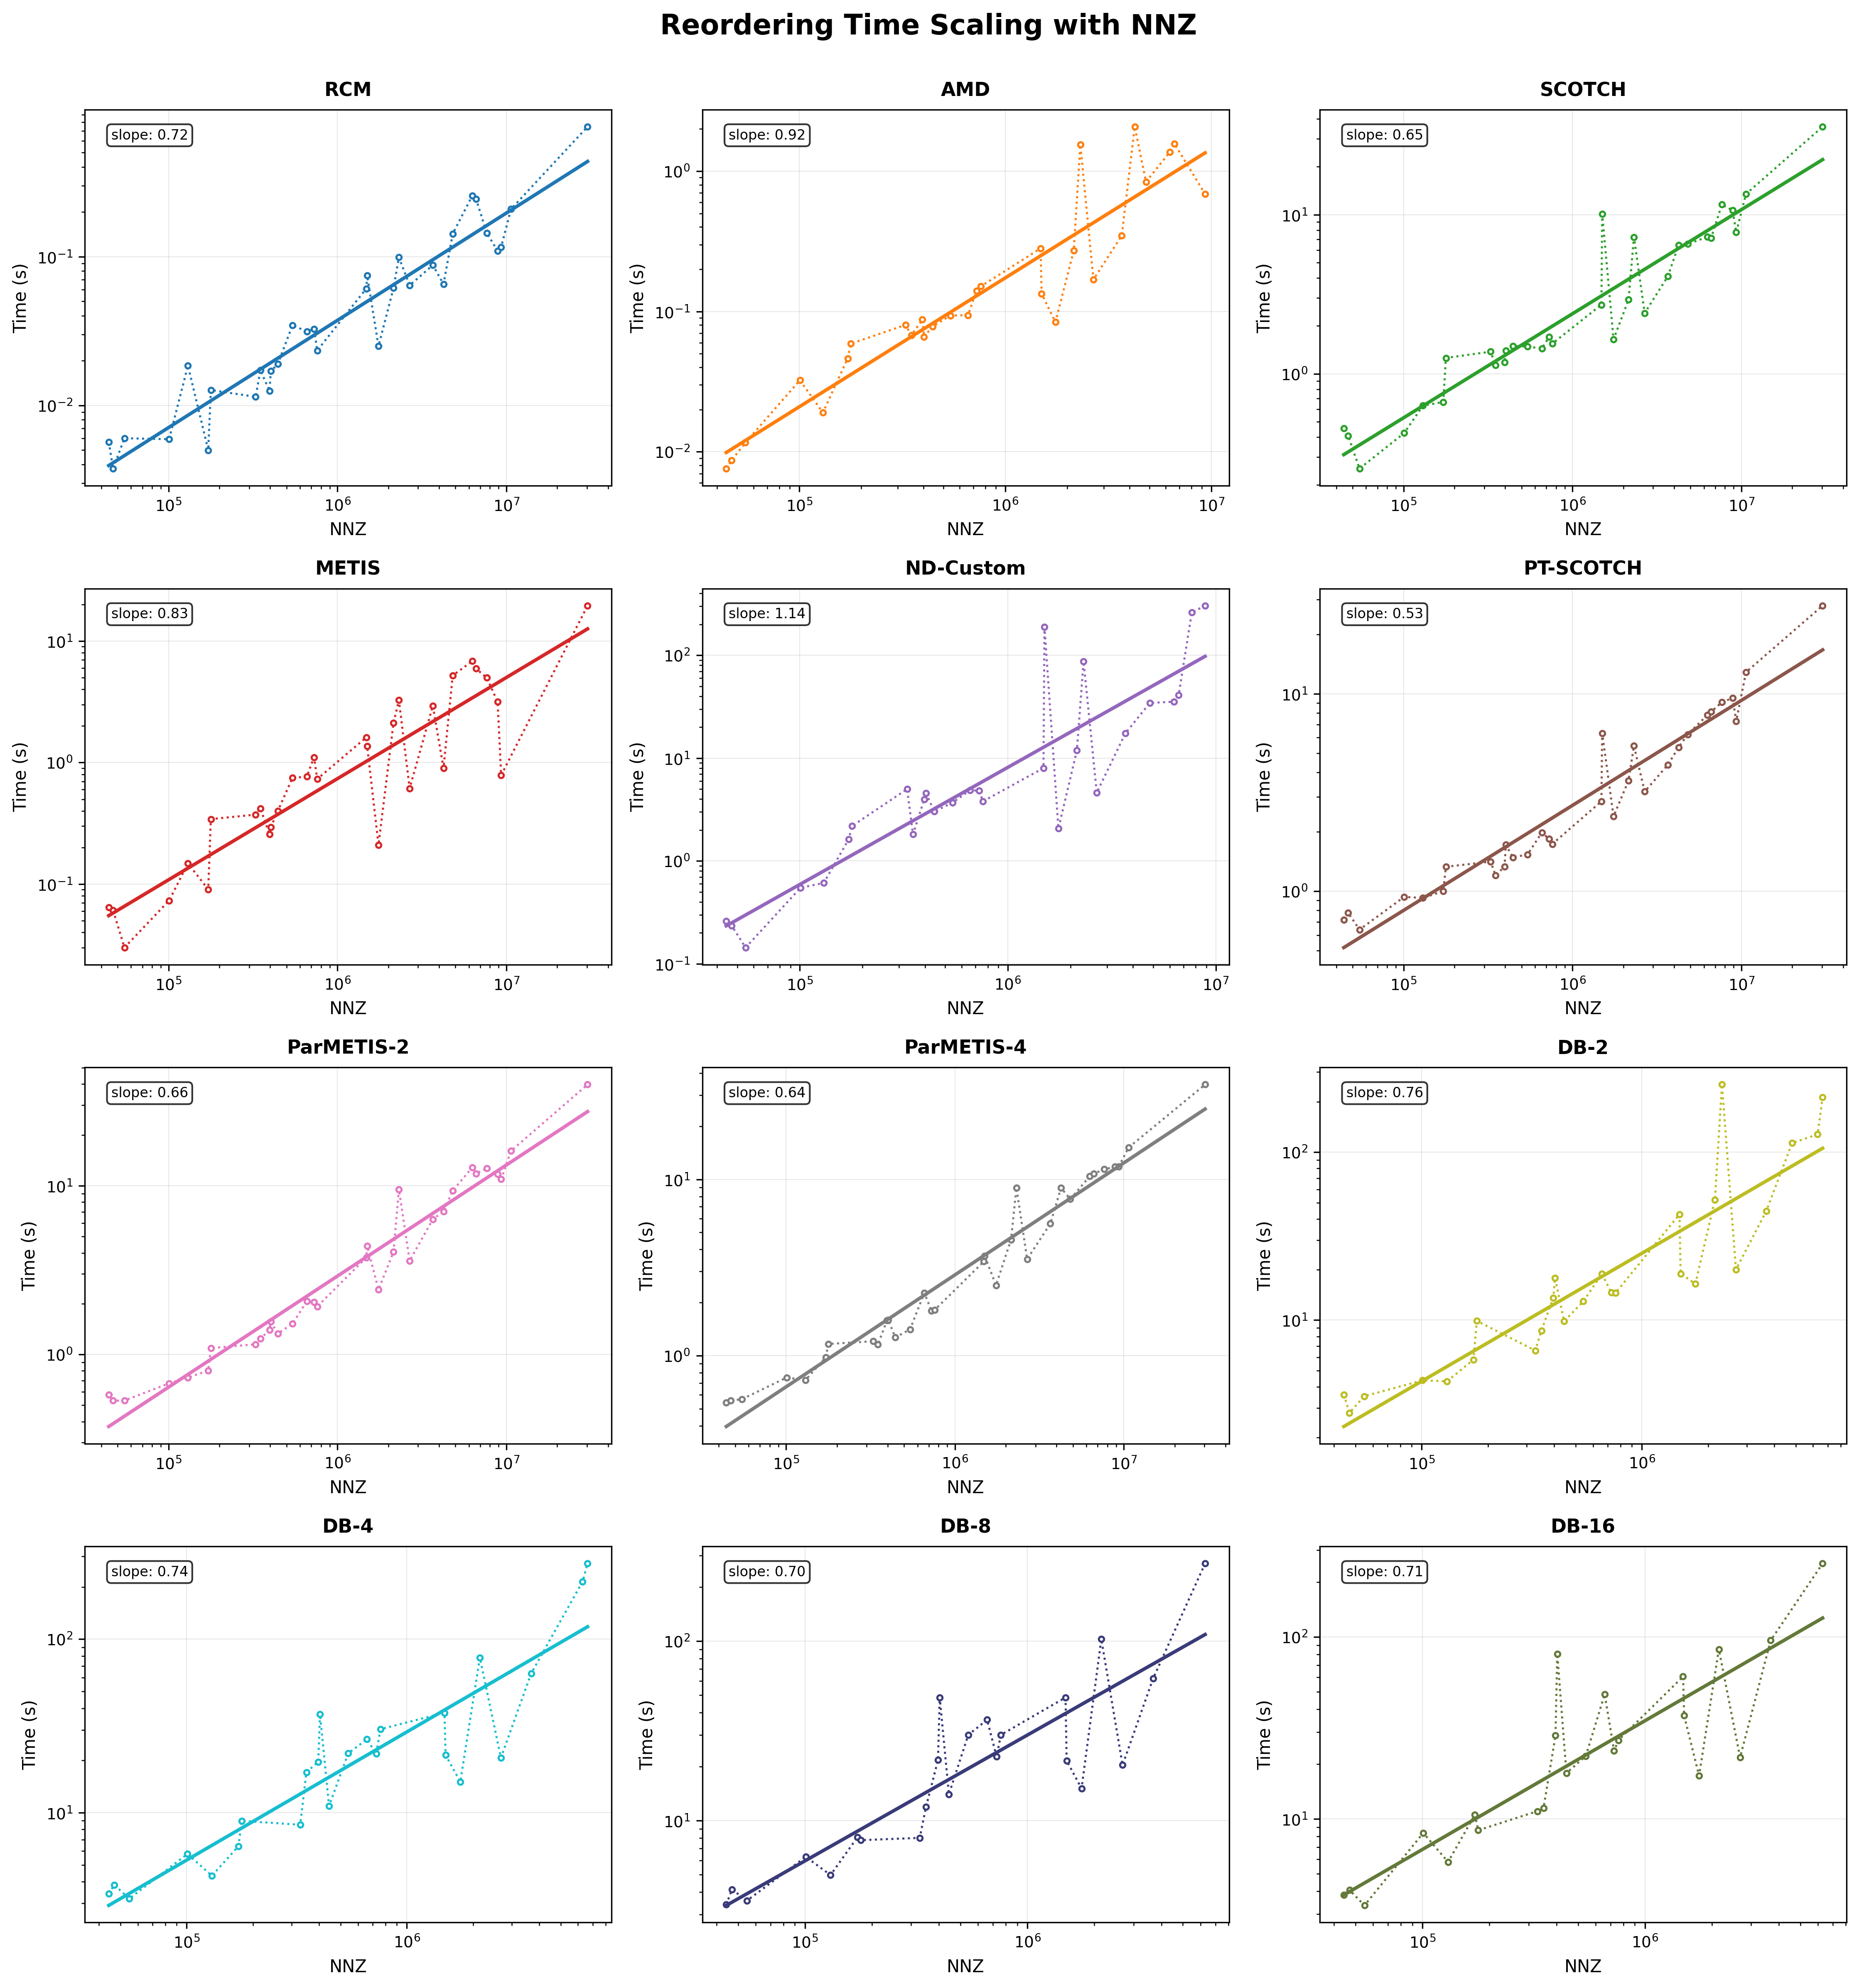
\includegraphics[width=\textwidth]{fig/res/reorder_time_scaling.png}
\caption{Reordering time scaling with matrix size (number of non-zeros) for different algorithms. Each subplot shows the relationship between matrix size and computational time for various reordering methods.}
\label{fig:reorder-time-scaling}
\end{figure}


\begin{figure}[h]
\centering
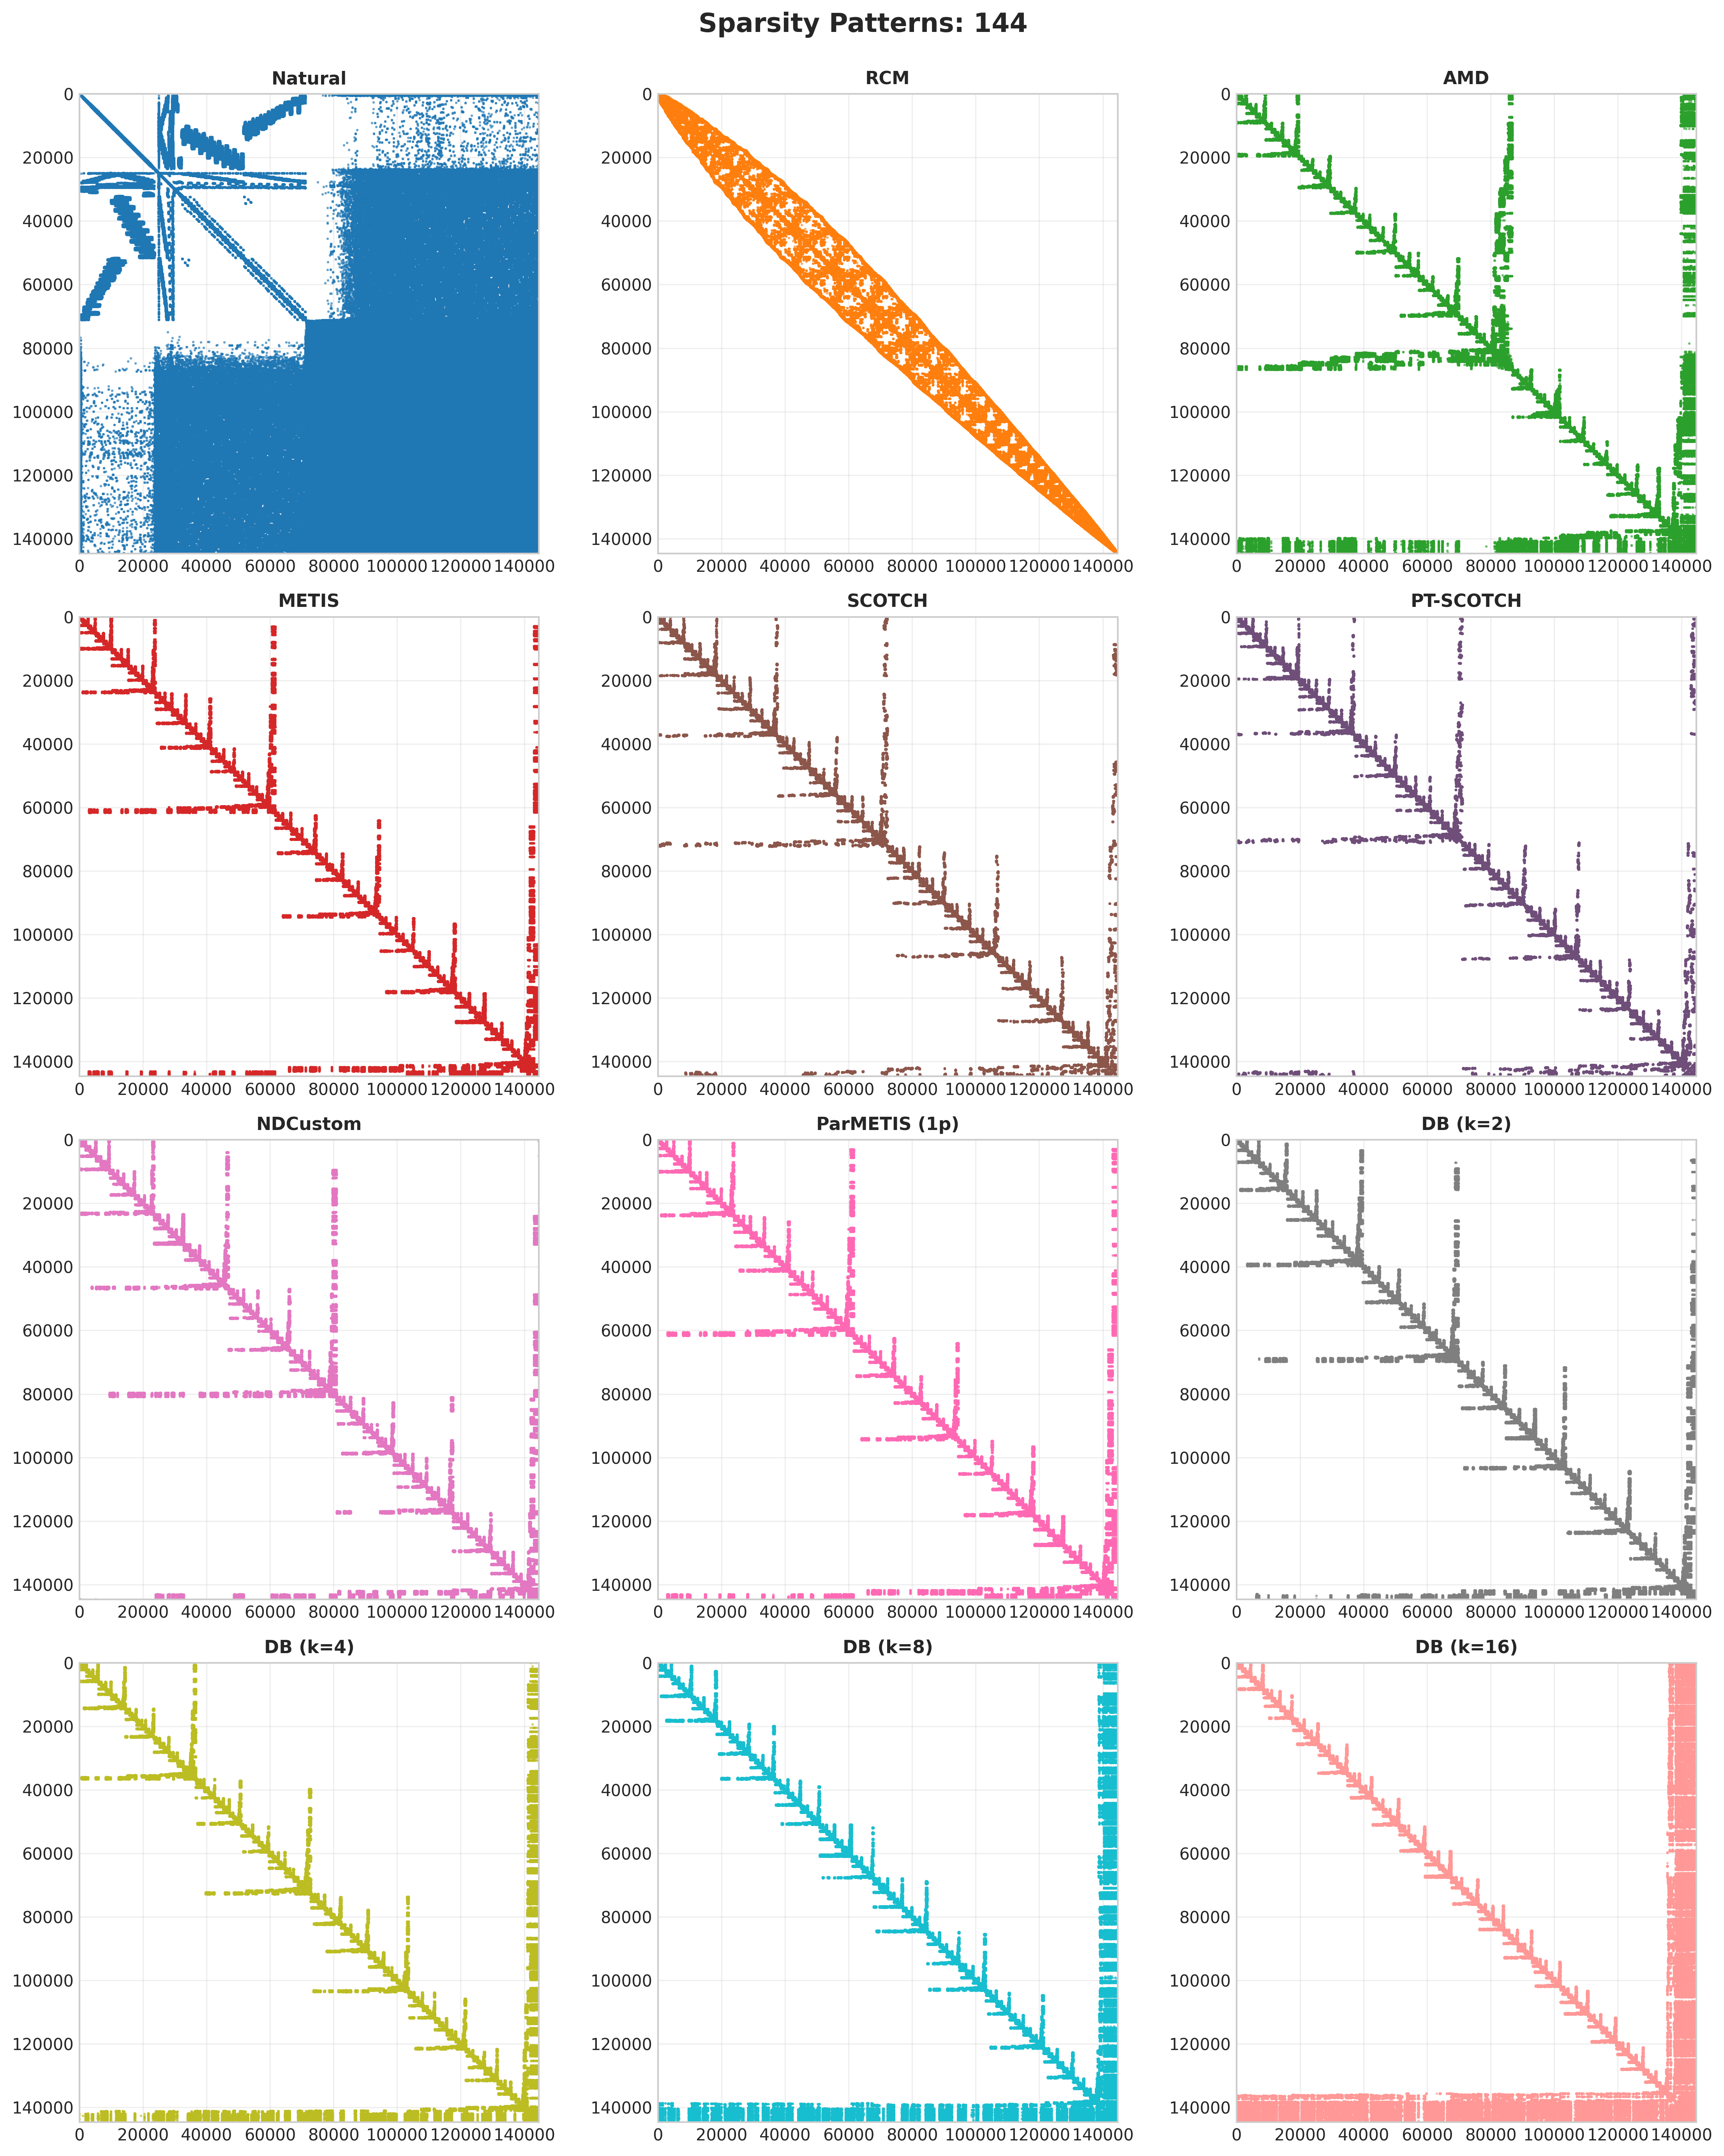
\includegraphics[width=\textwidth]{fig/res/144_sparsity_patterns.png}
\caption{Sparsity patterns of matrix 144 with different reordering algorithms applied. The natural ordering (top-left) shows a scattered pattern leading to high fill-in, while optimized reorderings (other panels) demonstrate more defined structures.}
\label{fig:144-sparsity-patterns}
\end{figure}

\begin{figure}[h]
\centering
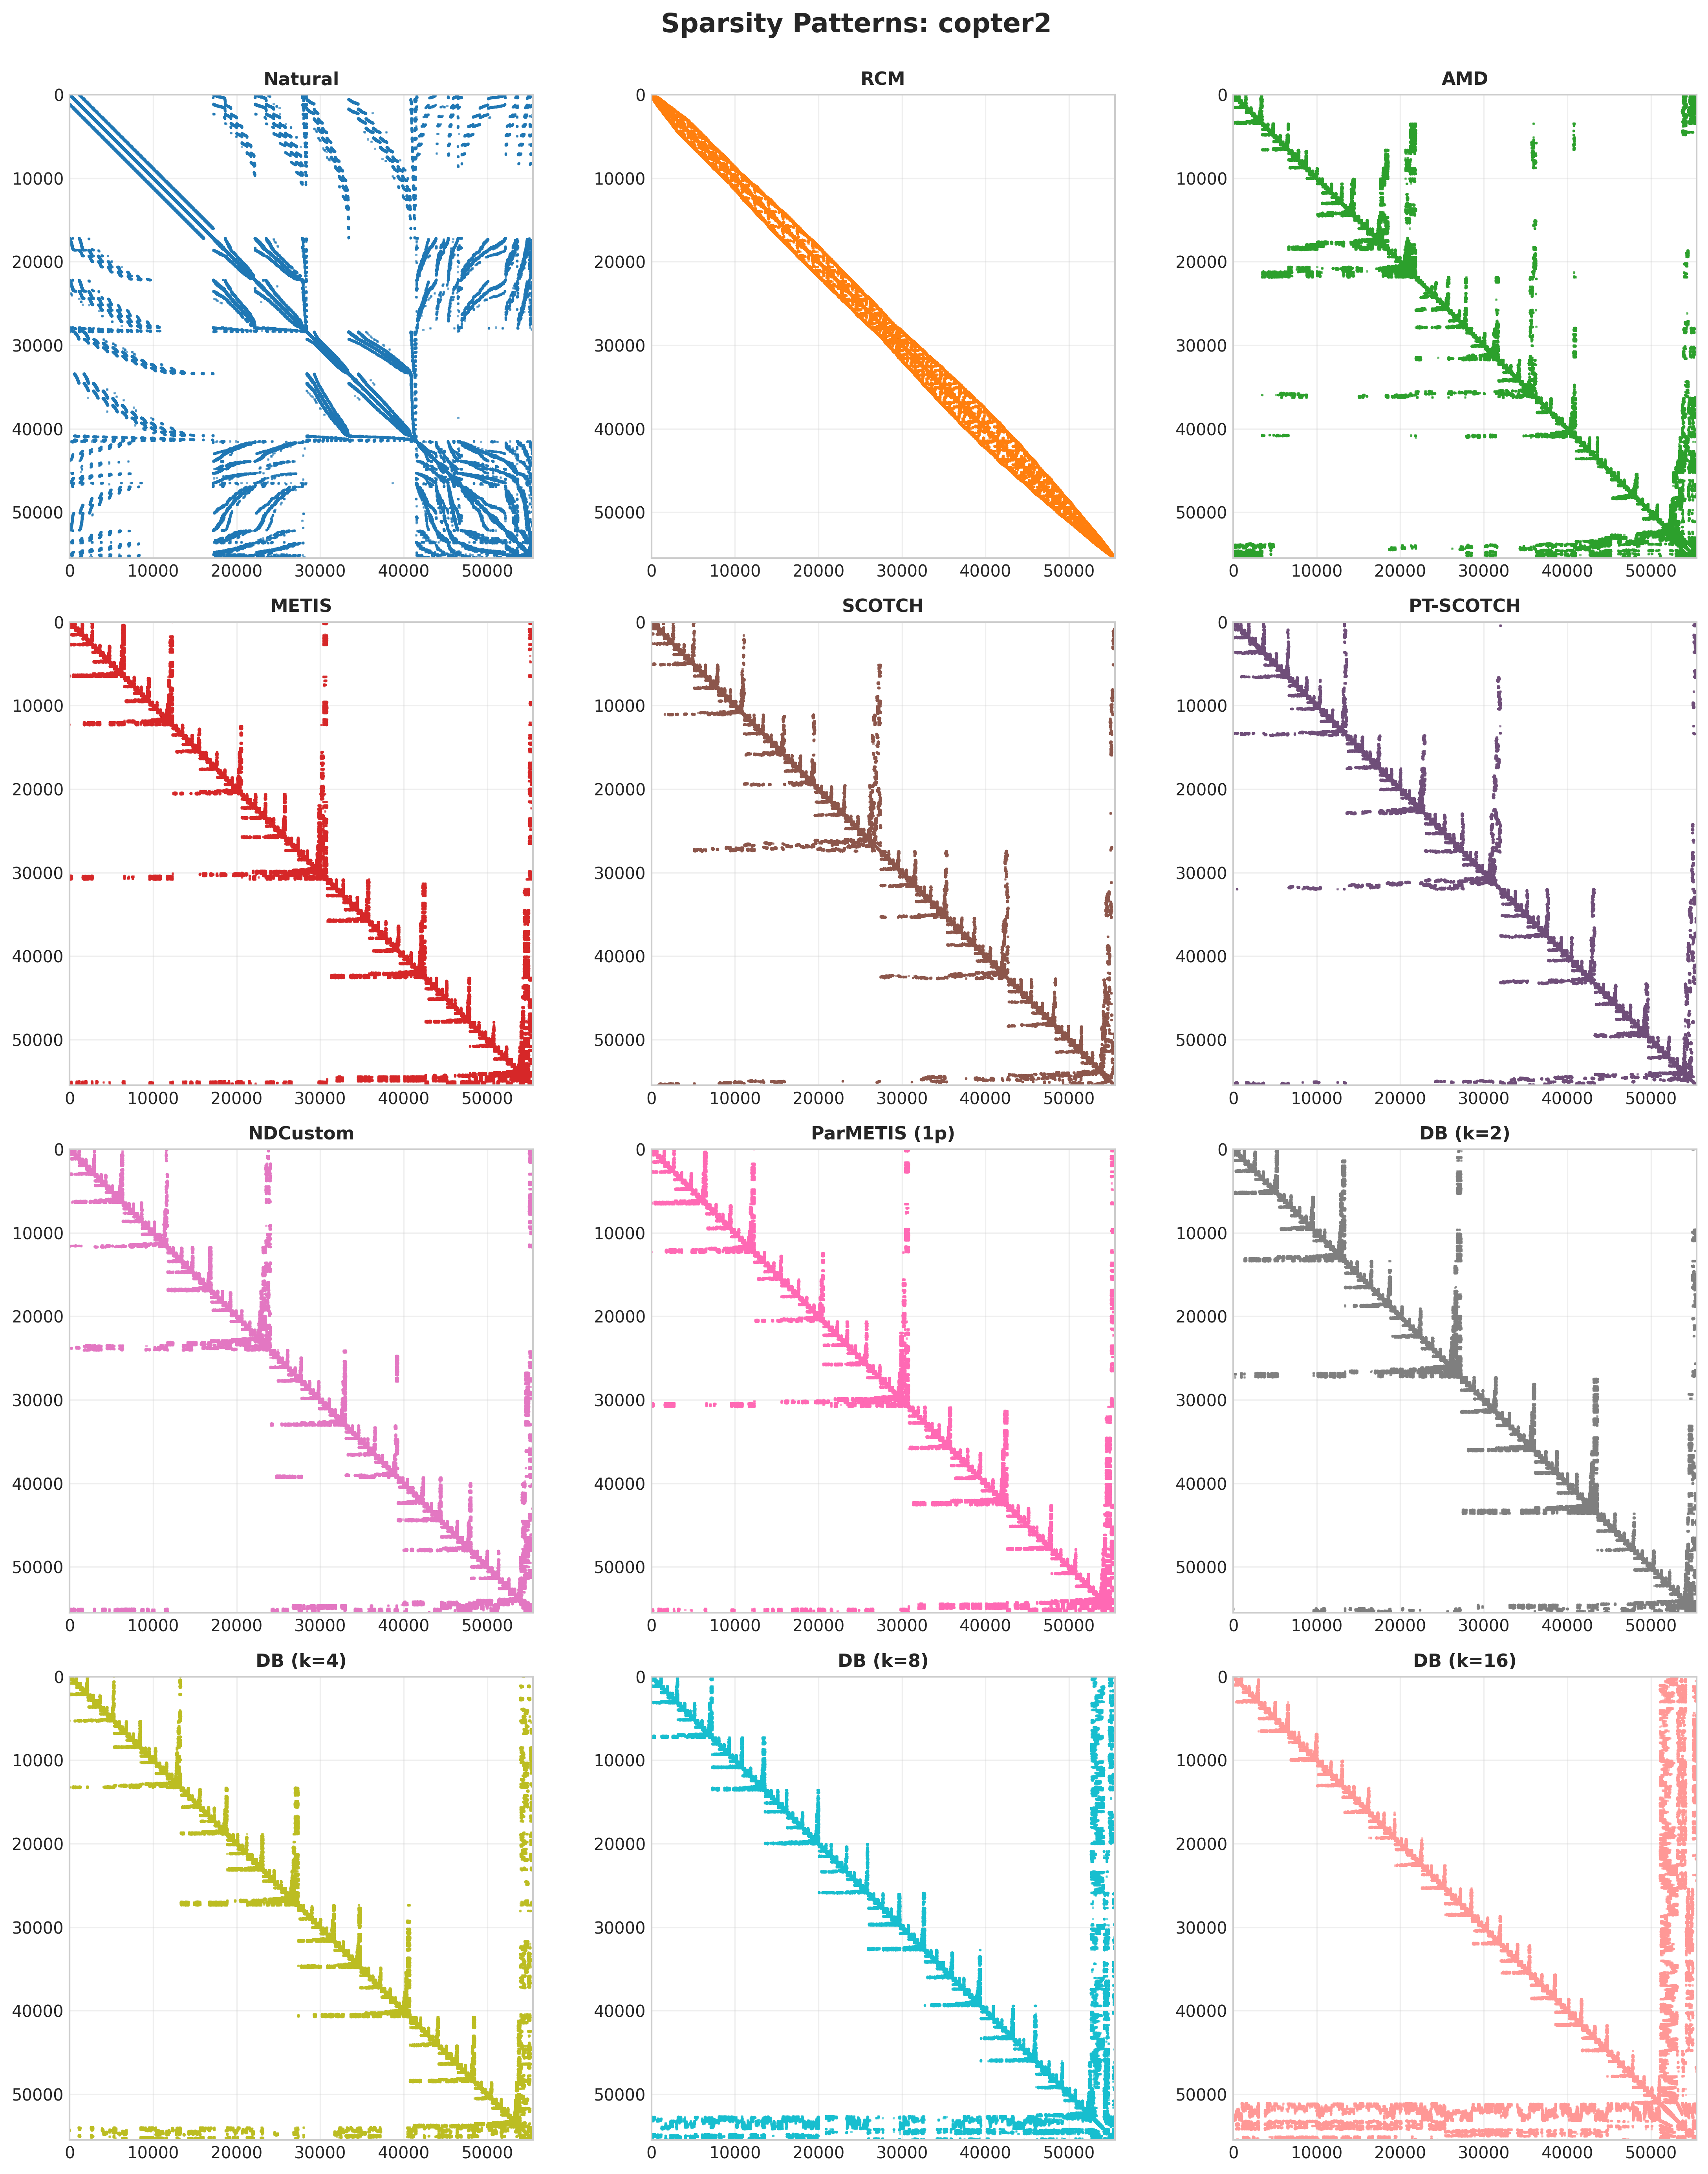
\includegraphics[width=\textwidth]{fig/res/copter2_sparsity_patterns.png}
\caption{Similarly, sparsity patterns of matrix copter2 with different reordering algorithms applied.}
\label{fig:copter2-sparsity-patterns}
\end{figure}

We then now look at the elimination tree depth as a measure of parallelism. Similar to fill-in, we sample randomly two matrices from different domains to show the elimination tree depth for different reordering algorithms.

The elimination tree depth results provide insight into the parallelization potential of different reordering methods, as shallower trees enable more parallel execution during factorization. The parallel methods show clear advantages in reducing tree depth compared to sequential approaches. ParMETIS variants consistently produce the shallowest elimination trees, with ParMETIS-2 and ParMETIS-4 often achieving depths in the range of 14-42 across various matrices, while ParMETIS-8 and ParMETIS-16 typically maintain depths between 25-50. METIS also performs well for parallelization potential, frequently producing trees with depths around 22-160, which represents a significant improvement over many sequential methods.

Sequential methods show mixed results for parallelization potential. AMD typically produces tree depths ranging from very shallow (4-20) for some matrices to quite deep (250-830) for others, making its parallelization benefits matrix-dependent. NDCUSTOM, being METIS with modified coarsening, generally produces similar tree depths to METIS, typically ranging from 24-171, though it can occasionally produce deeper trees (up to 839) for some matrices, suggesting that the coarsening modification does not consistently improve parallelization potential. RCM consistently produces the deepest trees, often exceeding 300-400 in depth and reaching over 700 for some matrices, which severely limits parallel factorization opportunities. SCOTCH performs moderately, with tree depths generally ranging from 23-290, while PT-SCOTCH shows improved parallelization potential with depths typically between 54-328, though it occasionally produces very deep trees exceeding 700.

The hypergraph partitioning methods (DB variants) show variable performance for parallelization, with tree depths ranging from 19-301 depending on the number of partitions used. DB-2 often produces deeper trees (49-603), while DB-16 tends toward moderate depths (66-830), though the relationship between partition count and tree depth is not always consistent. Natural ordering predictably produces very deep trees (often 200-800+), confirming the necessity of reordering for parallel factorization. The results indicate that while parallel reordering methods require more computational time, they provide substantial benefits for subsequent parallel factorization phases through significantly reduced elimination tree depths.


\begin{figure}[h]
\centering
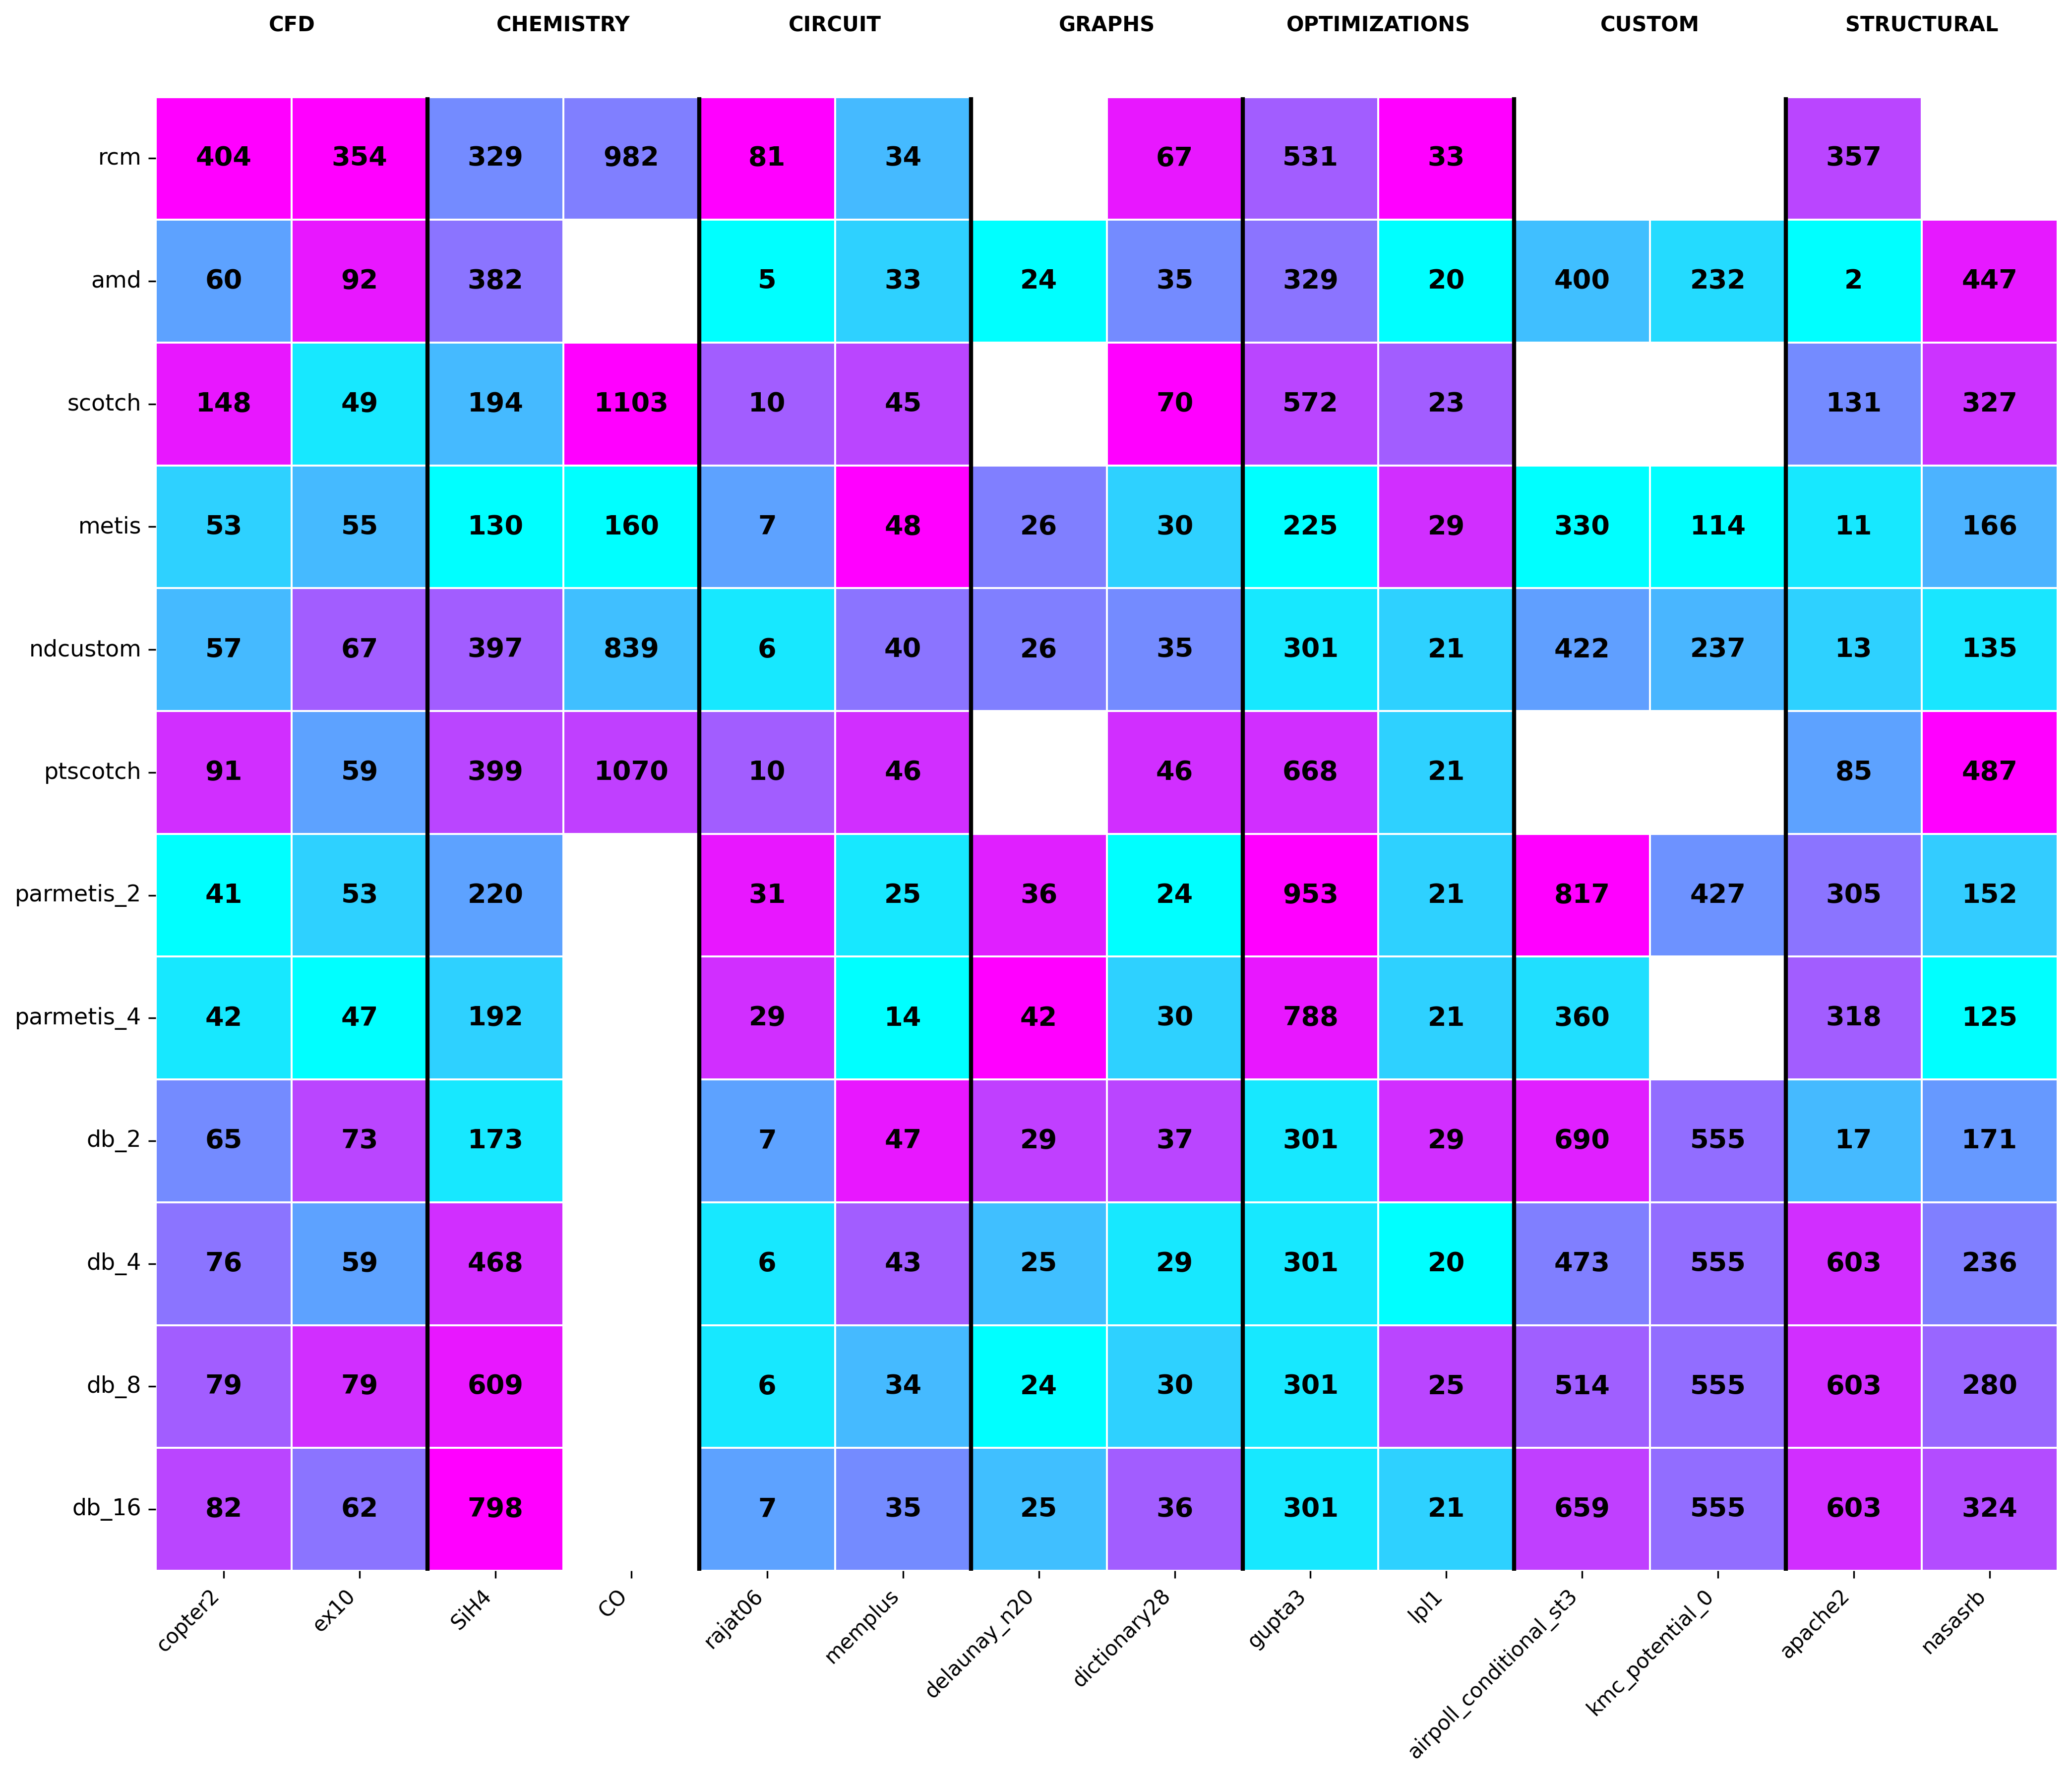
\includegraphics[width=1\textwidth]{fig/res/elimination_tree_depth_all_categories.png}
\caption{Elimination tree depth comparison across different matrix categories for various reordering algorithms. Lower depth indicates better parallelization potential. Blue indicates lower depth (better), while pink indicates higher depth (worse).}
\label{fig:elimination-tree-depth}
\end{figure}

\FloatBarrier

\subsection*{GPU-accelerated RCM}

In this section, we present the performance of our GPU-accelerated implementation of the Reverse Cuthill-McKee (RCM) algorithm compared to a traditional CPU-based implementation. We measure only the runtime of the RCM algorithm and not the fill-in, as the quality of the ordering produced by both implementations is identical.

\begin{figure}[H]
   \centering
   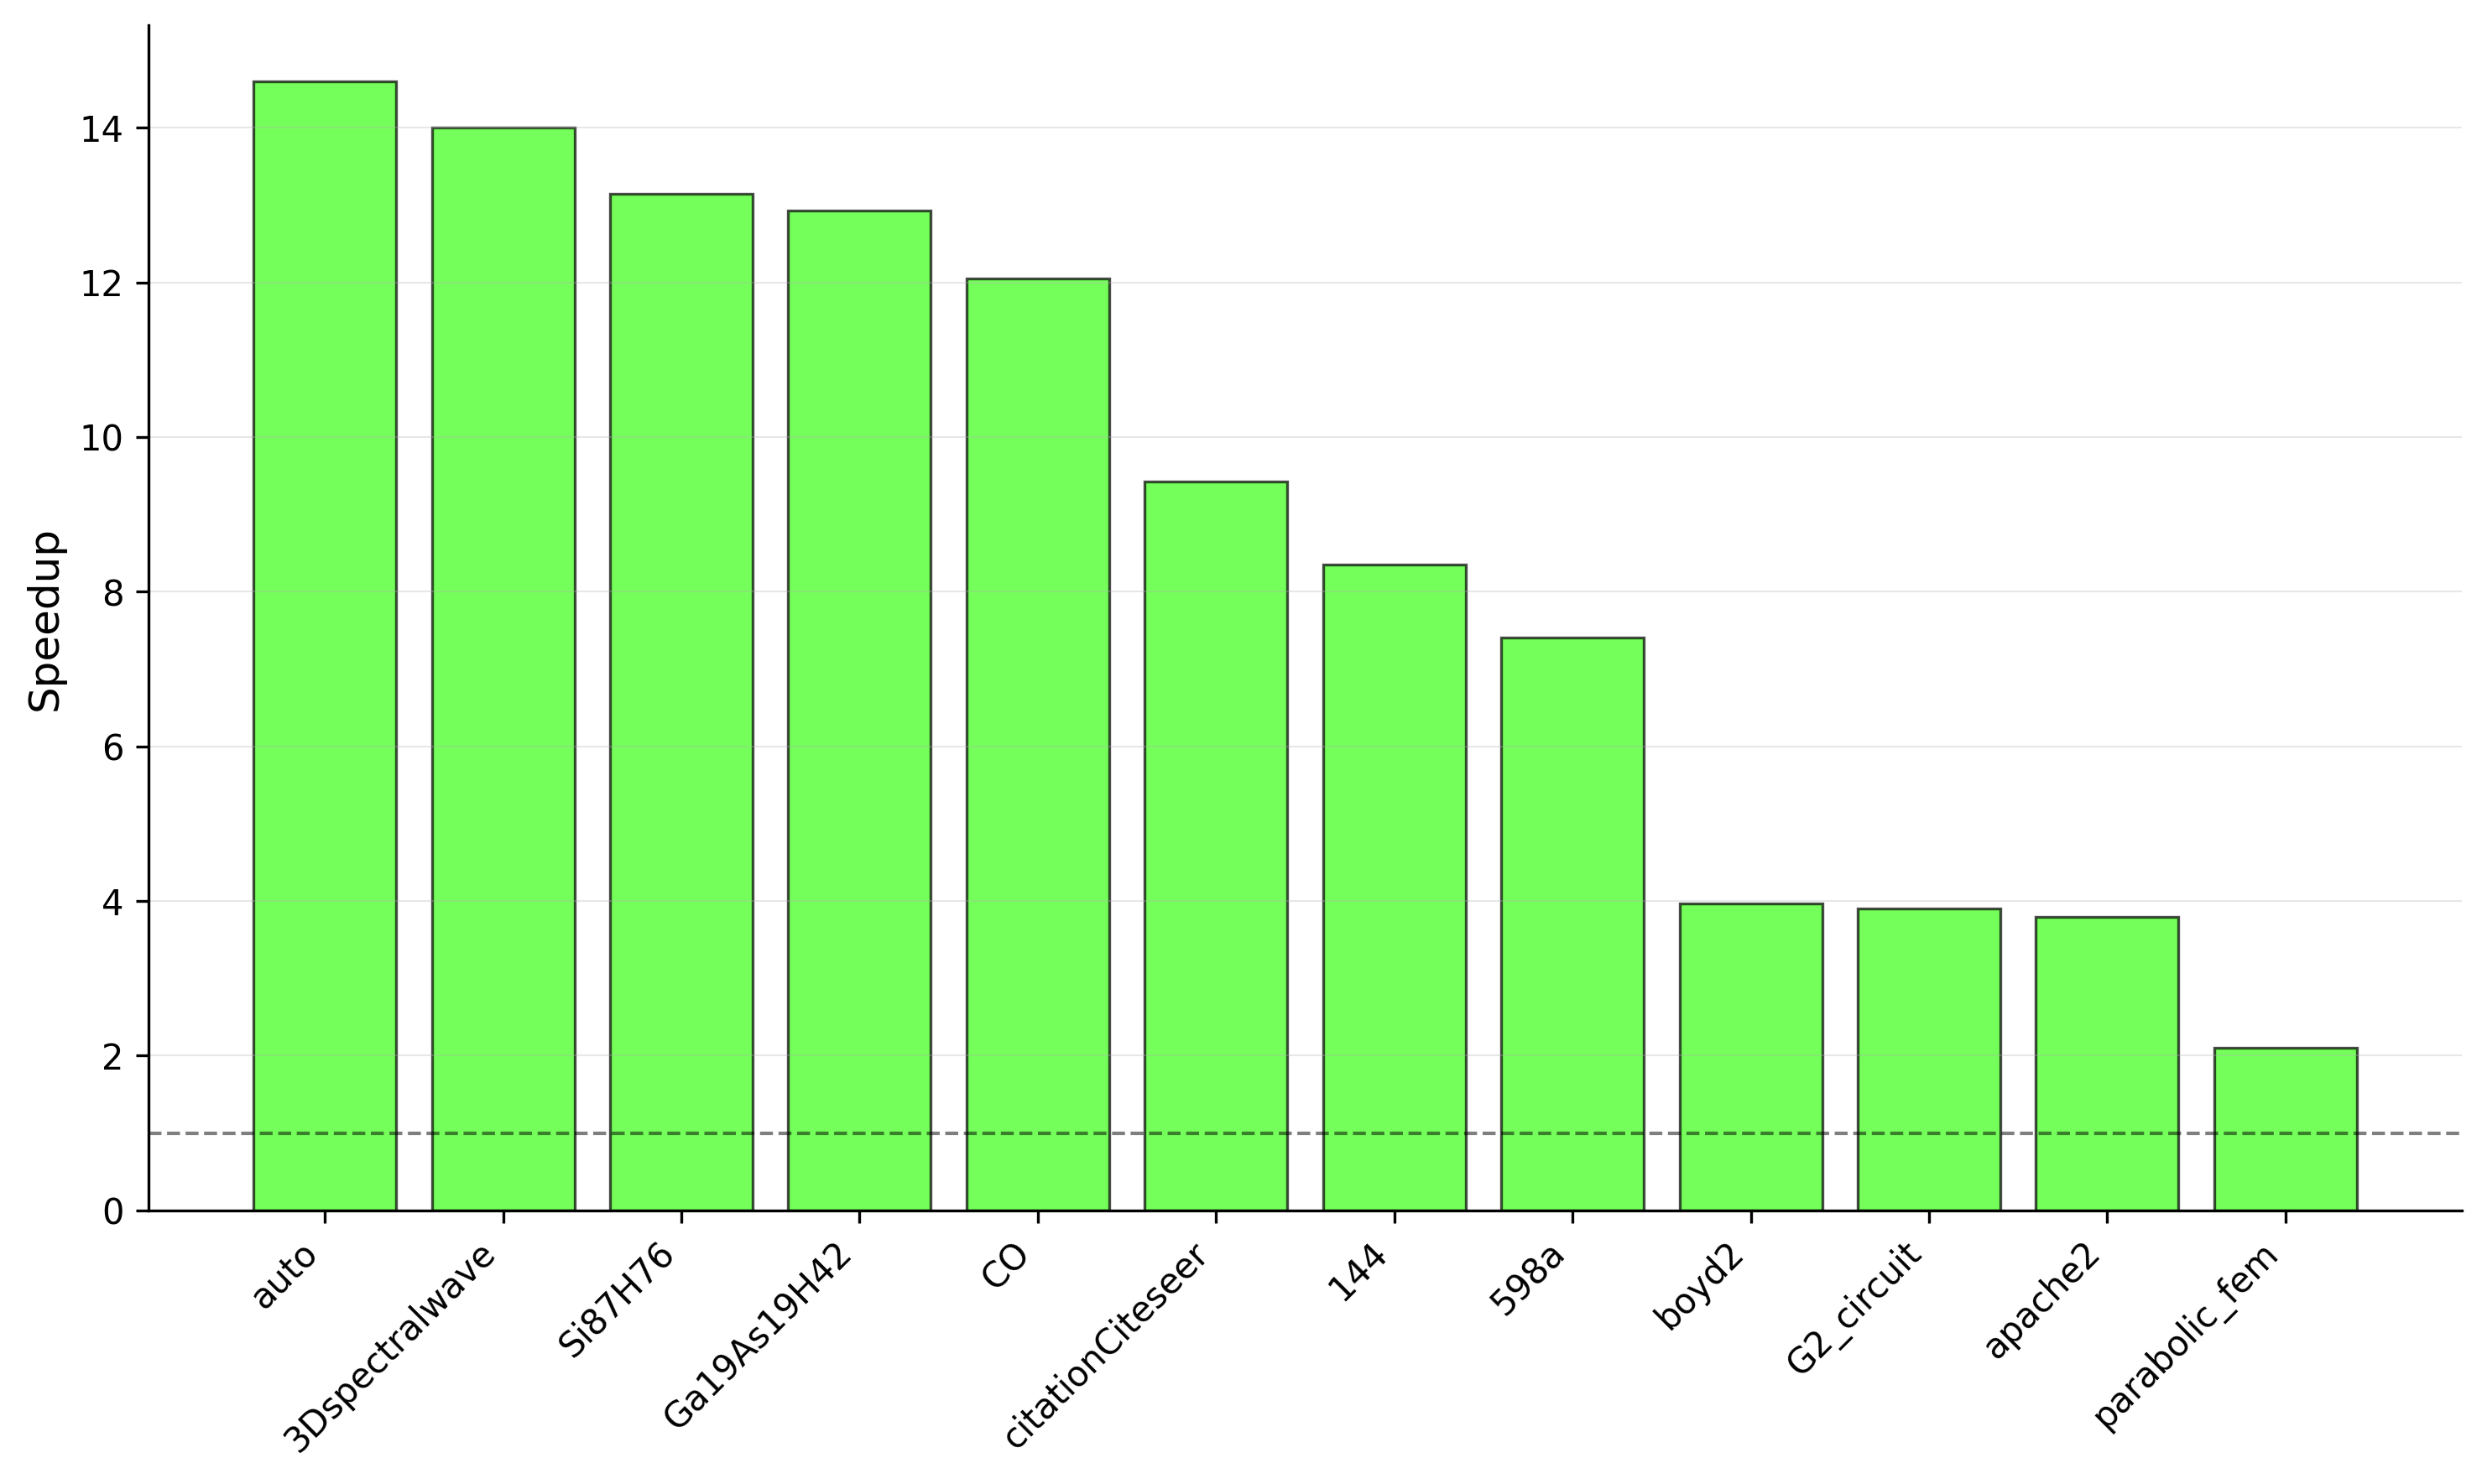
\includegraphics[width=0.9\textwidth]{fig/res/gpu_rcm_speedups_clean.png}
   \caption{Speedup of GPU-accelerated RCM compared to CPU-based RCM on large matrices (over 10K nodes).}
   \label{fig:gpu-rcm-speedups}
\end{figure}

\section{Current limitations}

Our evaluation has important limitations that should be acknowledged. First, our analysis is not exhaustive—we evaluated only a subset of available sparse matrix reordering algorithms and libraries, focusing on the most commonly used and representative methods. Additionally, our memory measurement system faced significant challenges: the monitoring thread frequently failed to capture meaningful data for fast-completing algorithms or when external binaries changed process IDs (particularly with hypergraph methods). For several large matrices, symbolic factorization failed due to memory constraints, preventing complete evaluation of all methods across our entire dataset.

The practical applicability of some methods is also limited by performance constraints. Hypergraph-based methods, while sometimes producing high-quality reorderings, proved computationally expensive and impractical for large matrices. Furthermore, our GPU acceleration efforts were limited to the RCM algorithm—we did not implement GPU versions of other reordering methods, which represents a significant opportunity for future performance improvements across the entire algorithm suite.


% Demonstrating that your implementation meets the objectives is usually done by showing a lower bound on a given figure of merit.
% Conversely, you should also illuminate the limitations of your implementation by showing upper bounds on these (or other appropriate) figures of merit.
% Critically examining your ideas and their implementation trying to find their limits is also part of your work!
